\documentclass[xcolor=table,mathserif,9pt]{beamer}    % ,handout
% colortbl only defines \rowcolor for a single row. xcolor extends this to multiple rows.

\usetheme{Aachen}
\usepackage[english]{babel}
\usepackage[utf8]{inputenc}
%\usepackage{tikz-dependency}
%\usepackage{chronology}
\usepackage{array, booktabs}
\newcommand{\foo}{\makebox[0pt]{\textbullet}\hskip+0.5pt\vrule width 5pt\hspace{\labelsep}}
\usepackage{multirow}
\usepackage{textcomp}
\usepackage{csquotes}
\usepackage{amsmath}
\usepackage[]{algorithm2e}
\usepackage{lipsum}
\usepackage{multicol}
\usepackage{hyperref}
\setlength{\columnsep}{1cm}
%%%%%%%%%%%%%%%%%%%%%%%%%%%%%%%%%%%%%%%%%%%%%%%%%%%%%%%%%%%%%%%%%%%%%%
% tables
\usepackage{multirow,array,tabularx,rotating}
\usepackage{booktabs}
\usepackage{tabularx}

% math
\usepackage{amsmath,amsthm, amssymb, latexsym, xspace}
%\usepackage{bbold}
\usefonttheme[onlymath]{serif}
\boldmath


% misc
\usepackage{subfigure}
\usepackage{wasysym}
\usepackage{nameref}
\usepackage{xcolor}
\usepackage{romannum}
% declare the path(s) where your graphic files are
\graphicspath{{./nlu/}{./g2p/}{./smt/}}
% and their extensions so you won't have to specify these with
% every instance of \includegraphics
\DeclareGraphicsExtensions{.pdf,.jpeg,.png}


%figures
\usepackage{tikz}
\usepackage{minibox}
% change the graphic extentions
%\usepackage{ifpdf}
%\ifpdf
%  \DeclareGraphicsExtensions{.pdf,.png,.jpg}
%\else
%  \DeclareGraphicsExtensions{.eps}
%\fi

\usepackage[np,autolanguage]{numprint}
\nprounddigits{1}

% helpers
\newcommand{\argmin}{\operatornamewithlimits{argmin}}
\newcommand{\argmax}{\operatornamewithlimits{argmax}}
\newcommand{\sign}{\operatornamewithlimits{sign}}
\newcommand{\Eqn}{Equation}
\newcommand{\Eqns}{Equations}
\newcommand{\Fig}{Figure}
\newcommand{\Figs}{Figures}
\newcommand{\Tab}{Table}
\newcommand{\Sec}{Section}
\def\example{{\textit{}{e.g.}}\xspace}
\def\cad{{\textit{}{i.e.}}\xspace}
\def\etc{{\textit{etc.}}\xspace}
\def\apriori{{\textit{a priori}}\xspace}

\newcommand{\NetTalk}{NETtalk\xspace}
\newcommand{\Celex}{Celex\xspace}
\newcommand{\Pronlex}{Pronlex\xspace}
\newcommand{\gtp}{G2P}
\newcommand{\Seg}{\mathbb{S}}
\newcommand\BLEU{\textsc{Bleu}\xspace}
\newcommand\TER{\textsc{Ter}\xspace}
\newcommand\CTER{\textsc{CTer}\xspace}

\newcommand\AER{\textsc{Aer}\xspace}
\newcommand\SAER{\textsc{Saer}\xspace}
\newcommand{\GIZA}{{GIZA\nolinebreak[4]\hspace{-.025em}\raisebox{.2ex}{\small\bf++}}\xspace}

\newcommand{\todo}[1]{\colorbox{yellow}{#1}\xspace}
\newcommand{\CITE}{\colorbox{yellow}{CITE}\xspace}
\newcommand{\REF}{\colorbox{yellow}{REF}\xspace}
\newcommand{\EQ}{\colorbox{yellow}{REF}\xspace}
\newcommand{\NUMBER}{\colorbox{yellow}{NUMBER}\xspace}
\newcommand{\Align}{\mathbb{A}}
%\renewcommand{\emph}[1]{\textcolor{i6blue}{#1}}


\newcommand{\aind}[1]{\hspace*{#1ex}}
\newcommand{\gray}[1]{\textcolor{gray}{#1}}

\newcommand*{\sumw}{\ensuremath{\operatornamewithlimits{sum}}\xspace}
\newcommand*{\nbest}{\ensuremath{\operatornamewithlimits{nbest}}\xspace}

% Define box and box title style
\usepackage{tikz}
\usetikzlibrary{shapes,positioning,fit}
\tikzstyle{bubble} = [ draw=blue, rectangle, rounded corners, inner sep=3pt, inner ysep=
10 pt]
\tikzstyle{fancytitle} =[fill=white, text=black]
\newenvironment{bubble}[3]{%
  \begin{tikzpicture}[transform shape, baseline=-0.5 cm]
  \def\bubbletitle{#1}%
  \node [bubble] (box)\bgroup
  \begin{minipage}[t][#3]{#2}%
}{%
  \end{minipage}%
  \egroup;
  \node[fancytitle] at (box.north) {\bubbletitle};
  \end{tikzpicture}%
}

\newenvironment{bubble*}[2]{%
  \begin{tikzpicture}[transform shape]
  \node [bubble] (box)\bgroup
  \begin{minipage}[t][#2]{#1}%
}{%
  \end{minipage}%
  \egroup;
  \end{tikzpicture}%
}

% CUSTOM STUFF %%%%%%%%%%%%%%%%%
%\usepackage{neuralnetworks}


% Rounding commands
\def\roundpositionii{1}
\newcommand{\rdmii}[1]{\edef\rounded{0}\FPeval\rounded{round(#1,\roundpositionii)}\rounded}
\def\roundpositioni{1}
\newcommand{\rdmi}[1]{\edef\rounded{0}\FPeval\rounded{round(#1,\roundpositioni)}\rounded}
\def\roundposition{0}
\newcommand{\rdm}[1]{\edef\rounded{0}\FPeval\rounded{round(#1,\roundposition)}\rounded}

\npstyleenglish

\def\roundposition{1}
\def\roundpositiont{3}
\edef\rounded{0}
\newcommand{\rd}[1]{\ifthenelse{\equal{#1}{--}}{--}{\edef\rounded{0}\FPeval\rounded{round(#1,\roundposition)}\rounded}}
\newcommand{\rdmt}[1]{\edef\rounded{0}\FPeval\rounded{round(#1,\roundpositiont)}\rounded}
\newcommand{\rp}[1]{%
  \FPset{\per}{#1}%
  %\FPmul{\per}{\per}{100}%
  \FPround{\per}{\per}{1}%
  \numprint{\per}%
}%


\setbeamercovered{transparent}

\DeclareMathOperator*{\sigmoid}{sigmoid}

\newcommand\T{\rule{0pt}{2.2ex}}       % Top strut
\usepackage{etoolbox}
\pretocmd{\section}{\addtocontents{toc}{\vspace{-20pt}}}{}{}

%Table stuff
\newcommand{\tablesize}{}
\newcommand{\abovetable}{\vspace{0.6cm}}
\newcommand{\belowtable}{\vspace{0.13cm}}


% Get fond size for system combination picture right
\usepackage{fix-cm}    
\makeatletter
\newcommand\SyscomFontSize{\@setfontsize\small{6}{60}}
\makeatother   

%%%%%%%%%%%%%%%%%%%%%%%%%%%%%%%%%

\newcommand{\backupbegin}{
   \newcounter{finalframe}
   \setcounter{finalframe}{\value{framenumber}}
}
\newcommand{\backupend}{
   \setcounter{framenumber}{\value{finalframe}}
}

\newcommand{\stoptocwriting}{%
  \addtocontents{toc}{\protect\setcounter{tocdepth}{-5}}}
\newcommand{\resumetocwriting}{%
  \addtocontents{toc}{\protect\setcounter{tocdepth}{2}}}

%%%%%%%%%%%%%%%%%%%%%%%%%%%%%%%%%%%%%%%%%%%%%%%%%%%%%%%%%%%%%%%%%%%%%%  
%%%%%%%%%%%%%%%%%%%%%%%%%%%%%%%%%%%%%%%%%%%%%%%%%%%%%%%%%%%%%%%%%%%%%%

\renewcommand*{\email}{\url{patrick.platen@rwth-aachen.de}}  
% all email address(es) of the authors (used for \TitlePage)

\title[Seminar]{ANN Supported Source Separation}
%\subtitle{Presentation Subtitle} % (optional)
%\setbeamertemplate{section in toc}[sections numbered] 
%\setbeamertemplate{subsection in toc}[subsections numbered] 
\setbeamertemplate{navigation symbols}{} %disable {, dotted}navigation bar

%% author and in []: shortauthorChange the scale of beamer from 3.5 to 1
\author[Patrick von Platen]{Patrick von Platen}
% - Use the \inst{?} command only if the author7s have different
%   affiliation.
\institute[RWTH Aachen University] % (optional, but mostly needed)
{
%  \inst{1}%
  \strut Human Language Technology and Pattern Recognition\\
  \strut Computer Science Department, RWTH Aachen University %\\
  %\strut {\tt lehnen@cs.rwth-aachen.de}
}
% - Use the \inst command only if there are several affiliations.
% - Keep it simple, no one is interested in your street address.

\date[19/6/2018]{June 19th, 2018}

%%%%%%%%%%%%%%%%%%%%%%%%%%%%%%%%%%%%%%%%%%%%%%%%%%%%%%%%%%%%%%%%%%%%%%shit
% will be set into the PDF document summary
\hypersetup{
  pdftitle={\inserttitle}, 
  pdfauthor={\insertauthor}, 
  bookmarksdepth=subsubsection,  
  % enable automatic page transitions: for endless loop edit in
  % acrobat reader -> preferences -> full screen -> after every X
  % seconds and after last page
  %pdfpageduration = 2, 
  % pdfpagetransition = {Glitter /Di 315 /D 5}  
  % pdfpagetransition = {Box /M /O /D 1},
} 
%%%%%%%%%%%%%%%%%%%%%%%%%%%%%%%%%%%%%%%%%%%%%%%%%%%%%%%%%%%%%%%%%%%%%%
%%%%%%%%%%%%%%%%%%%%%%%%%%%%%%%%%%%%%%%%%%%%%%%%%%%%%%%%%%%%%%%%%%%%%%

%%%%%%%%%%%%%%%%%%%%%%%%%%%%%%%%%%%%%%%%%%%%%%%%%%%%%%%%%%%%%%%%%%%%%%
%%%%%%%%%%%%%%%%%%%%%%%%%%%%%%%%%%%%%%%%%%%%%%%%%%%%%%%%%%%%%%%%%%%%%%
\begin{document}

%%%%%%%%%%%%%%%%%%%%%%%%%%%%%%%%%%%%%%%%%%%%%%%%%%%%%%%%%%%%%%%%%%%%%%
\begin{frame}[label=titlepage]
  \titlepage
\end{frame}

\begin{frame}
	\frametitle{Outline}
	\tableofcontents
        %\tableofcontents[currentsection, subsectionstyle=show/show/hide]
\end{frame}


%%%%%%%%%%%%%%%%%%%%%%%%%%%%%%%%%%%%%%%%%%%%%%%%%%%%%%%%%%%%%%%%%%%%%%




\section{Literature}%
\label{sec:literature}


\begin{frame}{Literature example}
2 pages
\begin{description}
\item [T.~Starner, J.~Weaver, A.~Pentland:] Real-time american sign-language recognition using desk and wearable computer based video. {\em PAMI 1998}.
  \begin{itemize}
  \item HMM based isolated sign language recognition. Explain the main content here.
  \end{itemize}
\item [Povey:] Papertitle. {\em ICASSP 2007}.
  \begin{itemize}
  \item something new in speech recognition. Explain the main content here.
  \end{itemize}
\item [\cite{BahdanauCB14}:] Papertitle. {\em CONFNAME 2007}.
  \begin{itemize}
  \item image retrieval. Explain the main content here.
  \end{itemize}
\end{description}
\end{frame}

\section{Introduction}%
\label{sec:introduction}
\begin{frame}{Source Separation}

\begin{center}
	\begin{figure}
	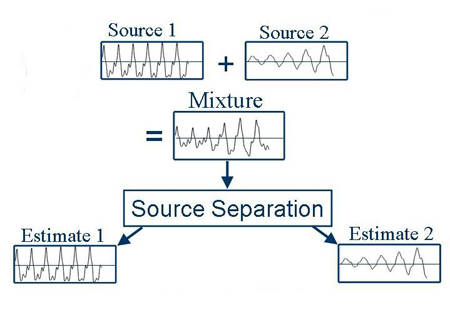
\includegraphics[width=.6\textwidth]{images/separation_example.jpg}
	\end{figure}
\end{center}

\textbf{Demo} \cite{Demo}
\begin{itemize}
	\item Mixture
	\item Source 1 
	\item Source 2 
\end{itemize}


\end{frame}

\begin{frame}{History \& Applications}

\begin{itemize}
	\setlength\itemsep{1em}
	\item History
	\begin{itemize}
		\item Cocktail party problem - first definition of source separation problem \cite{Cherry:1953} 
		\item Auditory scene analysis - first method for source separation \cite{bregman} 
		\item Computational scene analysis \cite{CASABrown} 
		\item Spectral Clustering \cite{Bach:2006} 
		\item Deep neural networks for speech separation \cite{SpeechSepDeepLearning:2015} 
		\item Deep Clustering \cite{DeepClustering2016}
		\item TasNet \cite{TasNet2017}
	\end{itemize}
	
	\item Applications
	\begin{itemize}
		\item Automatic meeting transcription 
		\item Virtual assistant
		\item Automatic subtitling of music/video
	\end{itemize}
\end{itemize}


\end{frame}

\section{Definition}%
\label{sec:definition}
\begin{frame}{Definition}

\begin{itemize}
	\setlength\itemsep{1em}
	\item Formal definition 
	\begin{itemize}
		\item Single-channel blind source separation
		\item No spatial information: Single channel
		\item No information about sources in advance: Blind
	\end{itemize}
	\item Mathematical definition
	\begin{itemize}
		\item Sources: $c = 1,...,C$
		\item Discrete time stepts: $t = 1,...,T$
		\item c-th source signal: $x_c(t)$
		\item Mixture: $X(t) = \sum_{c=1}^{C} x_c(t)$
		\item Goal: Recover $\{x_1(t),...,x_c(t)\}$ from $X(t)$
	\end{itemize}
\end{itemize}

\end{frame}

\section{Mathematical basics}%
\label{sec:mathematical_basics}
\begin{frame}{Short term fourier transform}

\begin{itemize}
	\setlength\itemsep{1em}
	\item Fourier transform 
	\begin{itemize}
		\item $S(f) = \int_{\mathbb{R}}X(t)e^{-2{\pi}jft}dt$
		\item Inverse Fourier transform: $X(t) = \int_{\mathbb{R}}X(f)e^{2{\pi}jft}df$
		\item Signal $X(t)$ can be decomposed to sum of weighted ``base frequencies''
		\item Fourier transform can be viewed as ``special convolution'' operation
	\end{itemize}
	\item Short term fourier transform
	\begin{itemize}
		\item Short term fourier transform: $S(f,t) = \int_{\mathbb{R}}X(\tau)w(\tau - t)e^{-2{\pi}jft}dt$ 
		\item Uncertainty in signal processing: Time localization vs. frequency precision
		\item Window function $w(\tau) = 0: \tau \not \in \left[-a, a \right]$ defines width of $(T,F)$ bins 
	\end{itemize}
\end{itemize}


\end{frame}

\begin{frame}{Spectrogram}

\begin{itemize}
	\item Shows the result of Short term fourier transform graphically
	\item Answers the question: \emph{Which frequencies are used at what time?}
\end{itemize}

\begin{center}
	\begin{figure}
		\includegraphics[width=.8\textwidth]{images/spectogram.png}
	\end{figure}
\end{center}

\end{frame}

\begin{frame}{Embedding}

	\begin{itemize}
		\item Structure-preserving, injective mapping $f: X \to Y$
		\item $Y$ is normed space: $d(y_1,y_2) \in \mathbb{R}, \forall y_1,y_2 \in Y$
		\item Example is \emph{word2vec}: 
			\begin{itemize}
				\item ``house'' $\to \left[1, 8, -8, 4, 5, 3, 29, -34\right]^{T}$
				\item ``car'' $\to \left[8,9, -8, 8, 5, 5, -34, -25\right]^{T}$
				\item Using euclidean distance norm: $d(f(\text{``house''}),f(\text{``car''})) = 64.19$ 
			\end{itemize}
		\item Mapping $f: X \to Y$ can be modelled using a neural network (see Deep Clustering)
	\end{itemize}



\end{frame}

\section{Conventional methods}%
\label{sec:conventional_methods}
\begin{frame}{Computational Auditory Scene Analysis \cite{CASABrown}}

\begin{algorithm}[H]
	\RestyleAlgo{boxruled}
	\LinesNumbered
	\emph{\textbf{Input: }}(N, $X(t)$) \\
	\emph{\textbf{Algorithm: }}
	\begin{enumerate}
		\item Segmentation:
			\begin{itemize}
				\item \small{ X(t) is transformed into (T,F) bins using STFT }
				\item (T,F) regions are defined using Segmenation rules 
			\end{itemize}
		\item Grouping:
			\begin{itemize}
				\item \small{ $(T,F)$ regions are combined to streams corresponding to sound sources}
				\item Auditory masks are created using different streams
			\end{itemize}
	\end{enumerate}
	\emph{\textbf{Output: }}$(\{x_1(t), ..., x_N(t)\})$
\end{algorithm}
	\vspace{10mm}
\begin{itemize}
	\item Motivated by Auditory Scene Analysis \cite{bregman}
	\item Model tries to imitate the human auditory system
	\item Segmentation \& grouping rules are f.e. based on:
	\begin{itemize}
		\item Rhythm, Periodicity, Proximity in frequency and time
		\item Common spatial location, Continuous or smooth transition
	\end{itemize}
\end{itemize}

\end{frame}

\begin{frame}{Spectral Clustering}
\begin{itemize}
	\item Similarity matrix $W \in \mathbb{R}^{P \times P}$ derived from dataset $D \in \mathbb{R}^P$
\end{itemize}
\vspace{10mm}
\begin{algorithm}[H]
	\RestyleAlgo{boxruled}
	\LinesNumbered
	\emph{\textbf{Input: }} $(W, k)$ \\
	\emph{\textbf{Algorithm: }}
	\begin{itemize}
		\item Compute first $k$ eigenvectors $U: (u_1,... ,u_k) \in \mathbb{R}^{P \times K}$ of $D^{-\frac{1}{2}}WD^{-\frac{1}{2}}$ with $D = \text{diag}(W)$
		\item Transpose $U$ to $V = U^T: (v_1,... ,v_p) \in \mathbb{R}^{K \times P}$ 
		\item Initialise \textbf{A} and perform K-means using $(v_1,... ,v_p)$ 
	\end{itemize}
	\emph{\textbf{Output: }}$\textbf{A} = (A_1, A_2, ..., A_k)$
\end{algorithm}
\end{frame}

\begin{frame}{Spectral Clustering for Source Separation \cite{Bach:2006}}
	
How to derive similarity matrix from mixed signal: \emph{$X(t) \to W$}?
\vspace{10mm}
\begin{enumerate}
	\item Short term fourier transform: $X(t) \to (F,T)$ bins
	\item Apply handcrafted features: \emph{Energy, continuity, common fate cues, pitch estimation, timbre}: $(F,T) \to (s_1, ...,s_n): n = F \times T$
	\item Create similarity matrix for every feature with $W_k(i,j) = f_k(s_i,s_j)$
	\item ``Concatenate'' similarity matrixes using weight vector $\alpha$: $W = W_1^{\alpha_1} \odot ... \odot W_k^{\alpha_k} \odot ...$ 
	\item Apply spectral clustering algorithm 
\end{enumerate}
\vspace{10mm}

\begin{itemize}
	\item $\alpha$ is trained using labeled data $\to$ \emph{Linear regression}
\end{itemize}


\end{frame}

\section{Problems with deep learning}%
\label{sec:problems_with_deep_learning}
\begin{frame}{Output dimension problem}

\begin{itemize}
	\item size(output layer) = \textbf{\#sources} $\times$ size(input layer)
\end{itemize}

\begin{figure}[htpb]
	\centering
	\includegraphics[width=0.8\linewidth]{images/outputDimProblem.png}
	\caption{Output dimension problem}
\end{figure}

\end{frame}

\begin{frame}{Output permutation problem}
	\begin{itemize}
		\item Label of speaker has to be assigned to ``matching'' part of output layer
	\end{itemize}

	\begin{figure}[htpb]
		\centering
		\includegraphics[width=0.8\linewidth]{images/permutationDimProblem.png}
		\caption{Output permutation problem}
	\end{figure}

\end{frame}

\section{Deep clustering}%
\label{sec:deep_clustering}
\begin{frame}{Deep clustering }

\begin{enumerate}
	\item $X(t) \to (F,T)$ bins
	\item $(f,t) \text{ bin } \to \text{ embedding }$ (encoding) via neural network
	\item Encodings are clustered via K-Means
\end{enumerate}

\begin{figure}[htpb]
	\centering
	\includegraphics[width=0.8\linewidth]{images/deepClustering.png}
	\caption{Deep clustering \cite{DCFigure}}
\end{figure}

\end{frame}

\begin{frame}{Deep clustering - Encoding}

 \begin{itemize}
	 \item $(F,T)$ spectogram $\in \mathbb{R}^{T \times F}$ is transformed to 
		 $s = (s_1, ..., s_n) \in \mathbb{R}^{N}$ with $N = T \times F$
	 \item Neural network: \emph{$f_{\theta}(s) = V$} with: 
		\begin{itemize}
			\item $\theta$ being the parameters of the neural network
			\item $|s|$ size of input layer
			\item $V \in \mathbb{R}^{N \times D}$ being the embedding
			\item Neural network has $D$ parallel output layers with 
			      of size $N$
		      \item $v_1, ..., v_n$ with \emph{$|v_i|^2 = 1$} normalized vectors
			      each representing an embedding of $(f,t)$ bin 
			\item $v_{i,1}, ..., v_{i,d}$ similar to handcrafted 
			      features in spectral clustering
		\end{itemize}
	\item $V$ is embedding of complete signal to be clustered
 \end{itemize}
\end{frame}

\begin{frame}{Deep clustering - Clustering}

\textbf{K-Means interference cost minimization}
\begin{itemize}
	\item $\min L = \sum_{i=1}^{N} ||s_i - \mu_k(i)||^2 = \sum_{k=1}^{K} \sum_{i \in C_k} ||s_i - \mu_k||^2$
\end{itemize}
\vspace{10mm}

\textbf{K-Means for Deep clustering}
\begin{itemize}
	\item $v_1, ..., v_n$ are clustered using K-Means
	\item \emph{$\hat{Y} = \text{argmin}_{Y} {V - Y(Y^TY)^{-1}Y^TV}$}
	\item $Y \in \mathbb{R}^{N \times C}$
	\item $Y = (y_1,... ,y_c): y_i \in \mathbb{R}^{N}$: ``K-Means center vectors'' $\to$ mask for $(F,T)$ bins
	\item $(Y^TY)^{-1}Y^T \in \mathbb{R}^{C \times N}$: means of all clusters
	\item Create masks \emph{$S_i = \hat{Y}(c) \odot s$}
	\item Output dimension problem is solved 
\end{itemize}
	
\end{frame}

\begin{frame}{Deep clustering - Training}
	
	\textbf{Minimize cost function $C(\theta)$}
	\begin{itemize}
		\item $C(\theta) = |VV^T - YY^T|_F^2$
		\item $Y$ is one-hot encoding from label $\overline{Y}$
		\item Frobenius norm: $|A|^2_F = \sum_{i,j} A(i,j)^2$ 
		\item $VV^T \in \mathbb{R}^{N \times N}$ estimated affinity matrix 
		\item $YY^T \in \mathbb{R}^{N \times N}$ labeled affinity matrix
		\item Intuitive derivation: $C(\theta) = \sum_{i,j}(v_i^T v_j - y_i^T y_j)^2 = ...  = \emph{\sum_{i,j; y_i = y_j} |v_i - v_j|^2 + \sum_{i,j} (v_i^T v_j)^2 - N}$
		\item Computational most efficient cost function: $C(\theta) = |V^TV|_F^2 - 2|V^TY| + |Y^TY|$
		\item Permutation invariant: $VV^T(i,j) = VV^T(j,i)$
	\end{itemize}
		
\end{frame}

\begin{frame}{Deep clustering - Training}
	
\begin{figure}[htpb]
	\centering
	\includegraphics[width=0.95\linewidth]{images/dcExample.png}
	\caption{[Lensson]}
\end{figure}

\end{frame}

\section{TasNet}%
\label{sec:tasnet}
\begin{frame}{TasNet}

\begin{figure}[htpb]
	\centering
	\includegraphics[width=0.8\linewidth]{images/tasNetAll.png}
	\caption{TasNet}
\end{figure}
\vspace{10mm}
\begin{itemize}
	\item Neural network is applied to \emph{chunks of raw signal}
\end{itemize}

\end{frame}

\begin{frame}{Encoding}

\begin{minipage}[t]{0.48\linewidth}
	\begin{figure}[htpb]
		\centering
		\includegraphics[width=0.9\linewidth]{images/tasNetEncoding.png}
	\end{figure}
\end{minipage}%
\hfill%
\begin{minipage}[t]{0.48\linewidth}
	\begin{itemize}
		\item Mixed signal $x$ is divided into $K$ chunks $x_k$ 
		\item Gated convolution is applied to $x_k$: 
		\emph{$w_k = \text{ReLu}(x_k * U) \odot \text{Sigmoid}(x_k * V)$}
	\end{itemize}
	\vspace{5mm}
	\begin{itemize}
		\item Signal as sum of base functions: $x = wB$
		\item Weight vector $w \in \mathbb{R}^{N}$ with $N$ = 
		      dimension of output layer
		\item Basis functions $B = (b_1, ...,b_n)$ 
		\item $w$ gives magnitude of basis functions $B$
		\item Gated convolution is \emph{$w = B^{-1}x$}
	\end{itemize}
\end{minipage}	



\end{frame}

\begin{frame}{Separation}

\begin{minipage}[t]{0.48\linewidth}
	\begin{figure}[htpb]
		\centering
		\includegraphics[width=0.7\linewidth]{images/tasNetSeparation.png}
	\end{figure}
\end{minipage}%
\hfill%
\begin{minipage}[t]{0.48\linewidth}
	\hfill
	\begin{itemize}
		\item weights $w$ are normalized $w \to \hat{w} = \frac{g}{\sigma} \odot (w - \mu) + b$ 
		\item $\sigma$ and $\mu$ are \emph{variance} and \emph{mean}
		\item $g,b$ are gain and bias vector
		\item Deep recurrent neural network outputs weight masks for every
			speaker: $M = (m_1, ...,m_k)  = f_{\theta}(w)$
		\item Size(outputLayer) = Size(inputLayer) $\times$ $\#$Speakers
		\item Output dimension problem is not solved in TasNet
	\end{itemize}
\end{minipage}	

\end{frame}

\begin{frame}{Decoding}

\begin{minipage}[t]{0.48\linewidth}
	\begin{figure}[htpb]
		\centering
		\includegraphics[width=0.7\linewidth]{images/tasNetDecoding.png}
	\end{figure}
\end{minipage}%
\hfill%
\begin{minipage}[t]{0.48\linewidth}
	\hfill
	\begin{itemize}
		\item $w_i = m_i \odot w$: separate weight vectors
		\item Deconvolution operation to get raw signal: $x_i = w_iB$ 
		\item $x_i = \text{deconv}_{\hat{\theta}}(w_i)$ with $\hat{\theta}$
		      parameters of deconvolutional layer
		\item Chunks of signal $x_k$ can individually be separated $\to$ 
		      very \emph{low latency time} when decoding
	\end{itemize}
\end{minipage}	

\end{frame}

\section{Comparison \& Results}%
\label{sec:results}
\begin{frame}{Comparison \& Results}

2 pages
\end{frame}

\section{Conclusion}%
\label{sec:conclusion}
\begin{frame}{Conclusion}

1 page
\end{frame}

\begin{frame}
  \frametitle{Fancy Table with overlay \only<2>{(WMT2016)} \only<1>{(IWSLT2013)}}
  \only<1>{
  \begin{center}
	\scalebox{0.9}{
\begin{tabular}{|l|cc|cc|cc|cc|}
    \hline
    IWSLT De-En & \multicolumn{2}{c|}{dev} & \multicolumn{2}{c|}{test} & \multicolumn{2}{c|}{eval11} &  \multicolumn{2}{c|}{alignment-test}\\             \hline
    Model & \BLEU\% & \TER\% & \BLEU\% & \TER\% & \BLEU\% & \TER\% & AER\% & SAER\%\\    
    \hline
    Attention-Based & 30.5 & 48.7 & 29.3 & 50.6 & 33.9 & 46.6 & 41.8  & 66.3 \\
     \hspace{3mm}+ method & \textcolor{i6bluedark}{31.5} & \textcolor{i6bluedark}{47.2} & \textcolor{i6bluedark}{30.3} & \textcolor{i6bluedark}{49.0} & \textcolor{i6bluedark}{34.3} & \textcolor{i6bluedark}{44.3} & \textcolor{i6bluedark}{35.4} & \textcolor{i6bluedark}{44.2} \\
    \hline
\end{tabular}
}
	\end{center}}
	\only<2>{
	\begin{center}
\scalebox{0.9}{
\begin{tabular}{|l|cc|cc|cc|}
    \hline
    WMT En-Ro & \multicolumn{2}{c|}{newsdev2016/1} & \multicolumn{2}{c|}{newsdev2016/2} & \multicolumn{2}{c|}{newstest2016} \\             \hline
    Model & \BLEU\% & \TER\% & \BLEU\% & \TER\% & \BLEU\% & \TER\% \\    
    \hline
    Attention-Based & 19.8 & 62.0 & 21.3 & 58.1 & 20.3 & 60.4 \\ 
    +GA & \textcolor{i6bluedark}{21.0} & \textcolor{i6bluedark}{61.1 } & \textcolor{i6bluedark}{23.6} & \textcolor{i6bluedark}{56.4} & \textcolor{i6bluedark}{21.8} & \textcolor{i6bluedark}{59.4} \\ 
    \hline 
    \hspace{3mm} +method + conv ($D=10$,$M=1$) & \textcolor{i6bluedark}{21.4} & \textcolor{i6bluedark}{60.1 } & \textcolor{i6bluedark}{24.7} & \textcolor{i6bluedark}{55.4} & \textcolor{i6bluedark}{22.3} & \textcolor{i6bluedark}{58.7} \\ 
    \hline 
\end{tabular}
}
	\end{center}}
	\vfill
	\begin{itemize}
	  \item Improves translation by an average of $0.8$ BLEU on IWSLT2013
	  \item Great improvement in AER and SAER
	  \item<only@2> Improves translation by an average of $1.7$ BLEU on WMT2016
	  \begin{itemize}
	    \item<only@2> Adding convolutional feedback gives an additional $0.6$ BLEU on average
	  \end{itemize}
	\end{itemize}
\end{frame}

\begin{frame}{Usefull \LaTeX\ beamer resources}
\begin{description}
\item [Media Files:] The package \texttt{media9} has several option for playing audio and video files
\item [Information about Beamer:] General information about using the beamer presentation mode of latex can be found here: \url{https://en.wikibooks.org/wiki/LaTeX/Presentations}
\item [Online Table Editor:] \url{https://www.tablesgenerator.com/}
\end{description}
\end{frame}

%%%%%%%%%%%%%%%%%%%%%%%%%%%%%%%%%%%%%%%%%%%%%%%%%%%%%%%%%%%%%%%%%%%%%%%%%%%%%%%%

\begin{frame}[label=finalSlide]
  \label{LastPage}%
  \begin{center}
    \vfill
    {\Large
    \textcolor{i6bluedark}{Thank you for your attention}
    }
%     \vfill
%     \inserttitle
    \vfill
    {\insertauthor}

    \vspace{10mm}
    \url{patrick.platen@rwth-aachen.de}
  \end{center}
\end{frame}

\nocite{*}

\stoptocwriting
\section{Appendix}
\resumetocwriting

%\backupbegin


%%%%%%%%%%%%%%%%%%%%%%%%%%%%%%%%%%%%%%%%%%%%%%%%%%%%%%%%%%%%%%%%%%%%%%%%%%%%%%%%
\section*{Appendix}



%%%%%%%%%%%%%%%%%%%%%%%%%%%%%%%%%%%%%%%%%%%%%%%%%%%%%%%%%%%%%

\begin{frame}[allowframebreaks]
  \centerline{Reference}
 %\bibliographystyle{ieeetr}
 \bibliographystyle{i6bibstyle}
 \bibliography{references}
\end{frame}

%\backupend

\end{document}
